%\begin{sidewaysfigure}
%  \begin{center}
%  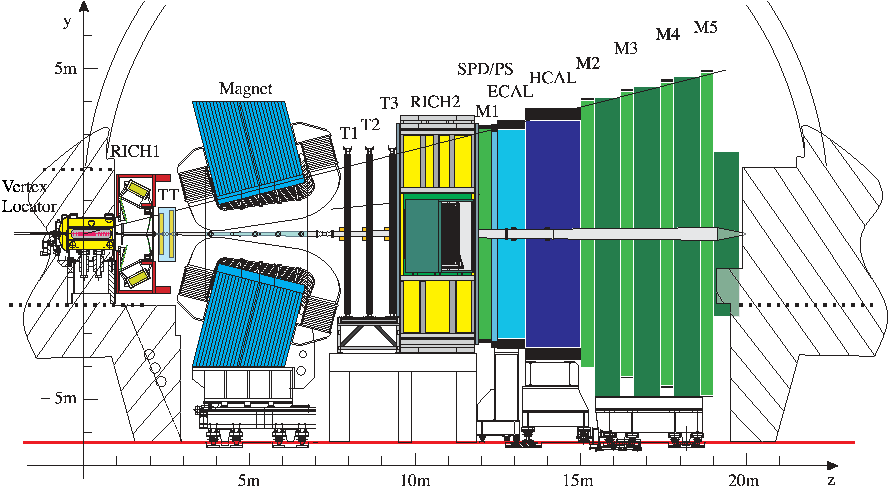
\includegraphics[width=0.8\textheight]{lhcb-detector-cross-section}
%  \caption[Cross-section view of \LHCb, cut in the non-bending $y$--$z$ plane]%
%    {Cross-section view of \LHCb, cut in the non-bending $y$--$z$ plane.}
%  \label{fig:LHCbCrossSection}
%  \end{center}
%\end{sidewaysfigure}



\chapter{Selection of neutrino interactions in the ECal}
\label{chap:NeutrinoInteractionSelection}
This analysis presents a measurement of the CC inclusive interaction cross-section of $\nu_\mu$ with lead nuclei using the ND280 tracker ECals.  To make such a measurement, a sample of neutrino interaction vertices within the ECal must be found.  The selection of events is based on the enhanced reconstruction outlined in chapter~\ref{chap:EnhancedECalReconstruction}.  However, as described in section~\ref{sec:ReconOutput}, the output of the enhanced reconstruction has been kept generic and isn't specifically tailored to this task.  The reconstruction's outputs a set of clusters which contain a set of 3D tracks and every pairwise crossing that said tracks make.  While it is true that in some situations the reconstruction will accurately represent a vertex out of the box, e.g. when only two tracks are reconstructed in the cluster, there will be many situations where extra reconstruction steps are needed before any further selection can take place.  After the final reconstruction steps have been discussed, a full discussion of the neutrino selection follows.

\section{Vertex reconstruction}
\label{sec:VertexReconstruction}
The output of the enhanced reconstruction already supplies most of the necessary information to reconstruct vertices in the ECal.  As a reminder, the reconstruction outputs a set of ECal clusters which contain the following:
\begin{itemize}
  \item A set of 3D reconstructed tracks
  \item The position at which every pairwise combination of 3D tracks most closely cross (pairwise crossings)
\end{itemize}
The reconstruction makes no quality checks on the 3D tracks in each cluster.  So, the first step is to remove any poorly reconstructed tracks from the cluster.  The need for this step is shown in Fig.~\ref{fig:AngularSeparationNoRejection} which shows the angular separation of reconstructed tracks with the simulated particle which created them, taken from beam Monte Carlo.  While the majority of tracks generally have a small angular separation, Fig.~\ref{fig:AngularSeparationNoRejection} clearly shows a build up of tracks which are offset by 90$^\circ$ to the simulated particles.
\newline
\newline
\begin{figure}%
  \centering
  \subfloat[No track rejection.]{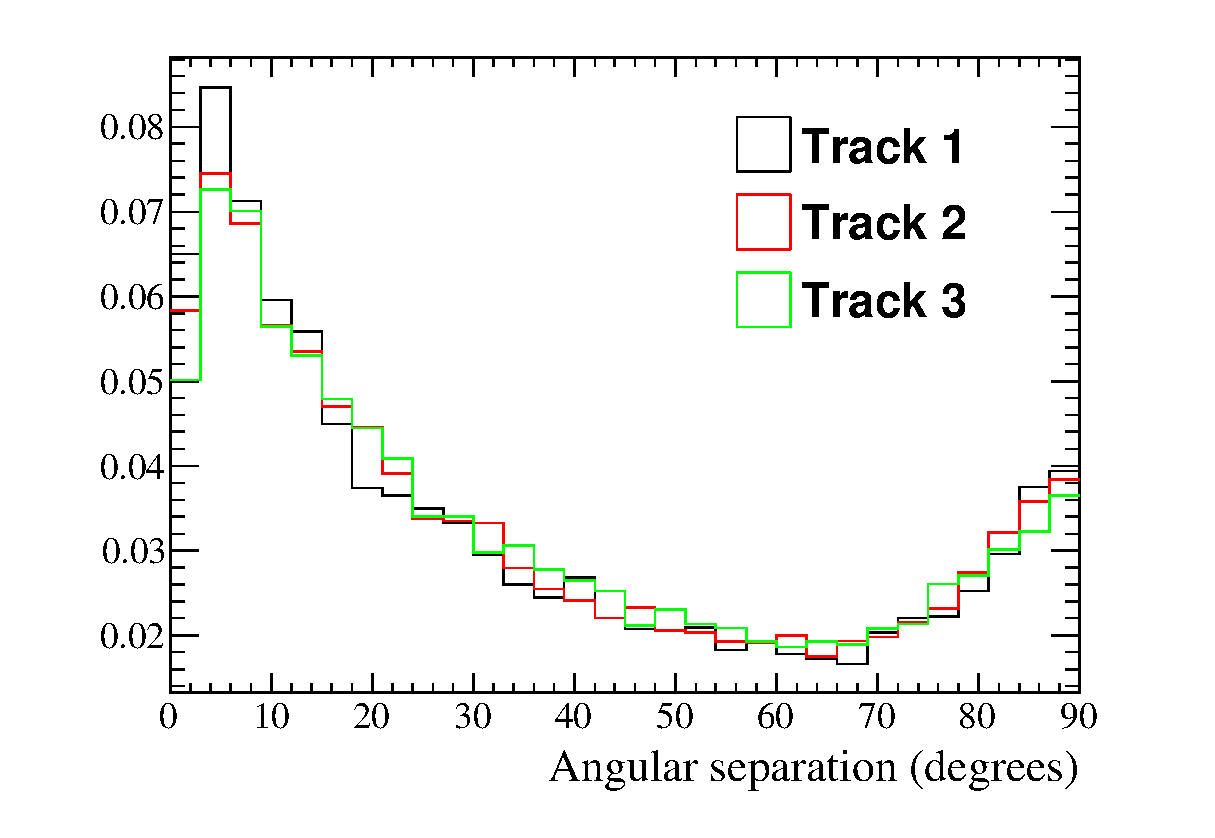
\includegraphics[width=9cm]{images/selection/track_rejection/AngularSeparationNoRejection} \label{fig:AngularSeparationNoRejection}}
  \subfloat[With track rejection.]{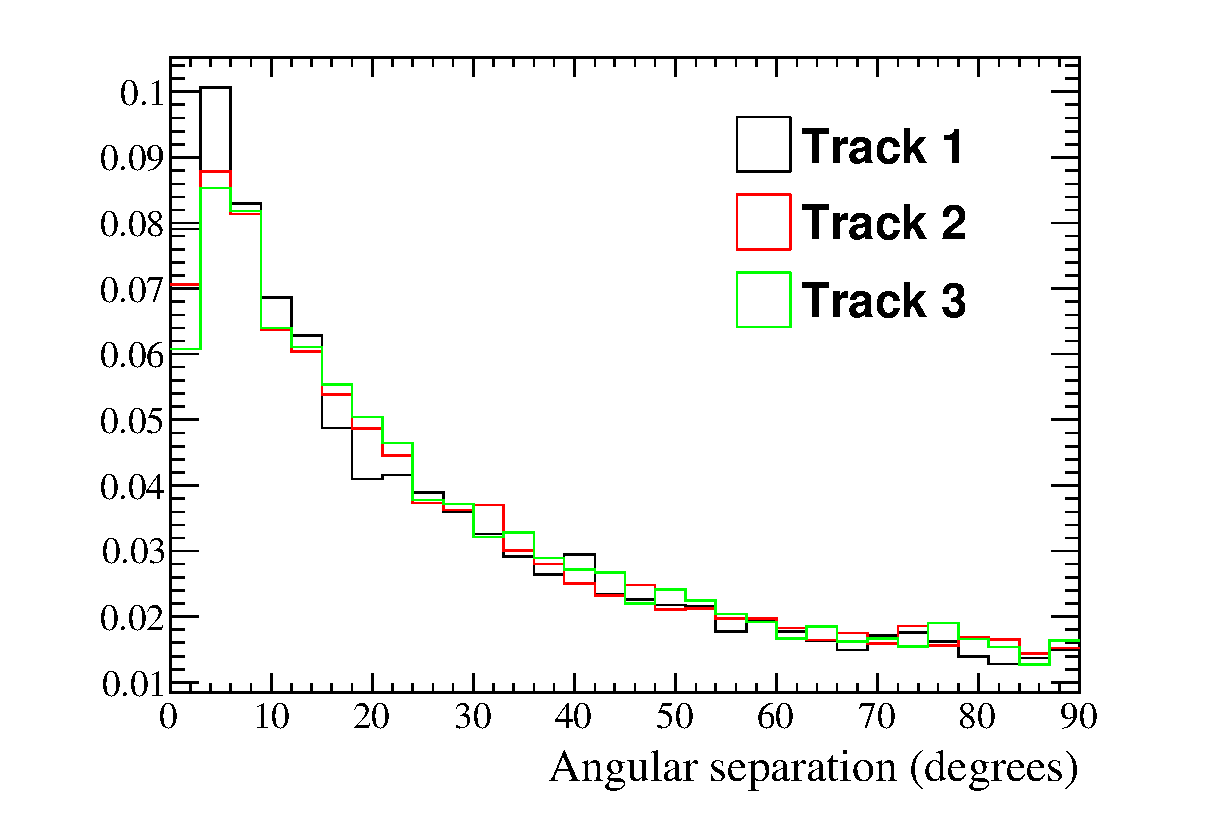
\includegraphics[width=9cm]{images/selection/track_rejection/AngularSeparationWithRejection}\label{fig:AngularSeparationWithRejection}}
  \caption{Angular separation of the reconstructed tracks in an ECal cluster with the beam-simulated particle that created them.  The black, red and green histograms are the tracks that were reconstructed first, second and third respectively.  All histograms are area normalized.}
  \label{fig:TrackRejectionAngularSeparation}
\end{figure}
There are two catagories of bad track reconstruction.  The first is where the 3D matching matches two 2D tracks which do not have sufficient information to fully model a 3D track.  Specifically, one of the 2D tracks involved in the matching only uses one ECal layer.  As the 3D track reconstruction requires information from both ECal views, tracks which fall into this catagory do not supply enough information to reconstruct a good quality track.  The second catagory is where the 3D matching produces a grossly incorrect match.  The matcher is designed to continually match 2D tracks together until no more 2D tracks are left in the matching pool.  So, there are situations where the last possible match made is in no way suitable.  This situation is easily indentified by matched 2D tracks which do not overlap.  For example, one of the 2D tracks uses layers 16, 18 and 20 and the other 2D track uses layers 1 and 3.  By removing these two types of tracks from the cluster, the 90$^\circ$ build up in the angular separation distribution is surpressed, as shown in Fig.~\ref{fig:AngularSeparationWithRejection}.  By removing these catagories of tracks, approximately 22$\%$ of tracks are rejected.
\newline
\newline
The final states of a neutrino interaction originate from the same point in space.  So, assuming that the reconstructed tracks represent the final states, the reconstructed tracks should most closely cross at the point of interaction.  As stated above, one of the outputs of the reconstruction are the pairwise crossings of the constituent tracks in the ECal cluster.  Using the above assumptions,  the pairwise crossings should be in close proximity to one another when the reconstructed tracks represent the final states of an interaction.  This idea promotes a relatively simple method of vertex reconstruction: attempt to cluster the pairwise crossings together if the pairwise crossings are in close proximity.  To quantatively define this proximity, the quality of the pairwise crossing also has to be considered.
\newline 
\newline
As with the 3D tracks, the reconstruction does not perform any quality checks on the pairwise crossings of the tracks.  As the reconstruction will always find a crossing location for a pair of 3D tracks, some of the pairwise crossings will not represent anything physical.  The quality definition chosen is simple: pairwise crossings are defined as bad if the crossing location is far away from either of the tracks it is associated with.  However, the distance definition is not trivial to define and should be closely correlated with the vertex reconstruction method.  For example, a two track vertex would provide very little constraint on the distance which defines a bad crossing, whereas a three track vertex may provide a bad crossing distance constraint which is too strict and destroys the majority two track vertices. 
\newline
\newline
The above discussion promotes two parameters which will govern the vertex reconstruction: the required proximity of two crossings to be clustered together, $d_c$, and the distance of a crossing from its constituents tracks to be classified as bad quality, $d_q$.  To quantify these values, a sample of reconstructed events matched to interactions in the ECals are used which are taken from beam Monte Carlo.  The reconstruction (the pairwise crossing rejection and clustering) is repeatedly run over the sample for different values of the $d_c$ and $d_q$ to find the optimum values.  To define the optimum value, a figure of merit is necessary.  After running the reconstruction for a given $d_c$ and $d_q$, the number vertices are separated into one, two and three track vertices and the true neutrino interactions which created the reconstructed vertices are associated.  A reconstructed vertex is tagged as correctly reconstructed if it contains the same number of reconstructed tracks as the number of charged final states in the associated neutrino interaction.  By defining the number of correctly reconstructed one, two and three track vertices as $N_1$, $N_2$ and $N_3$ respectively, the figure of merit, $\phi^{\textrm{vertices}}$, is
\begin{equation}
  \phi^{\textrm{vertices}} = N_1N_2N_3.
\end{equation}
\begin{figure}
  \centering
  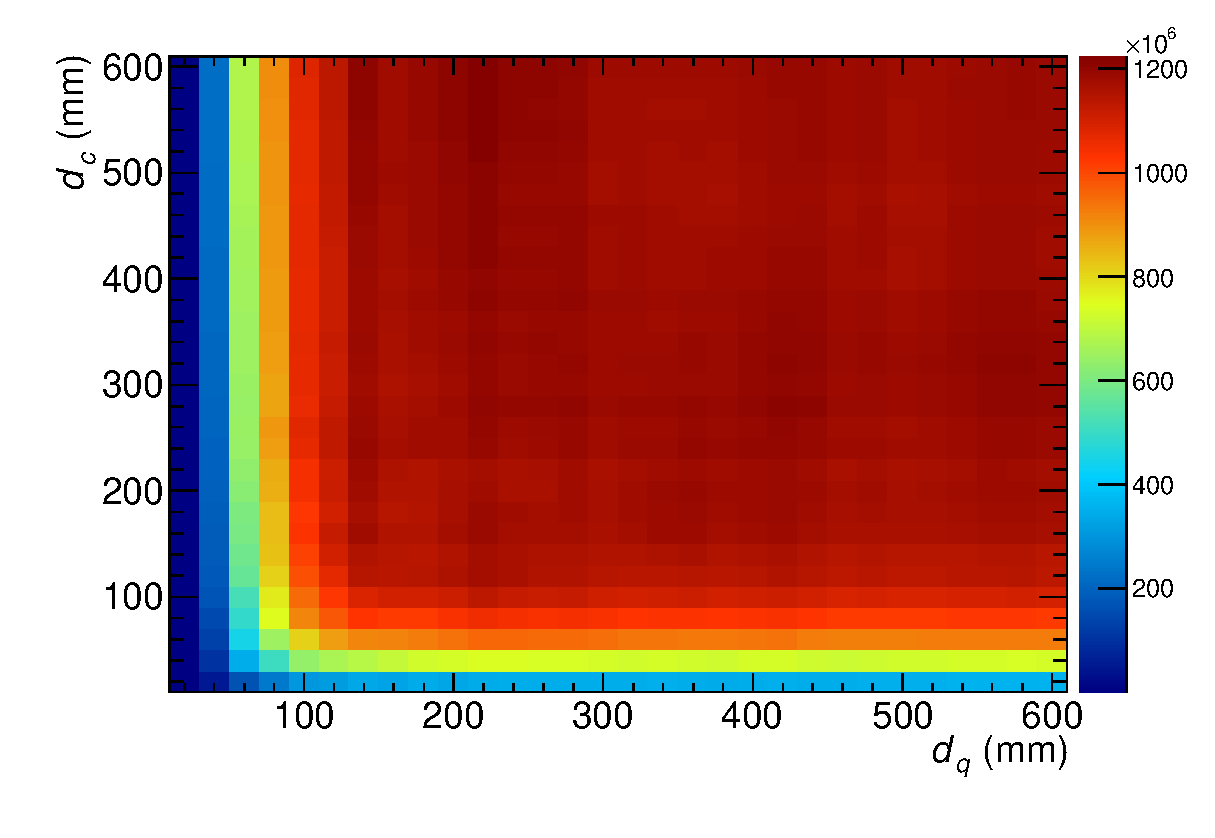
\includegraphics[width=12cm]{images/selection/vertex_recon/FOM_2D}
  \caption{Values of $\phi^{\textrm{vertices}}$ in ($d_q$,$d_c$) space.  The colour corresponds to the magnitude of $\phi^{\textrm{vertices}}$.}
  \label{fig:VertexReconFOM}
\end{figure}
\begin{figure}
  \centering
  \subfloat[$d_q$]{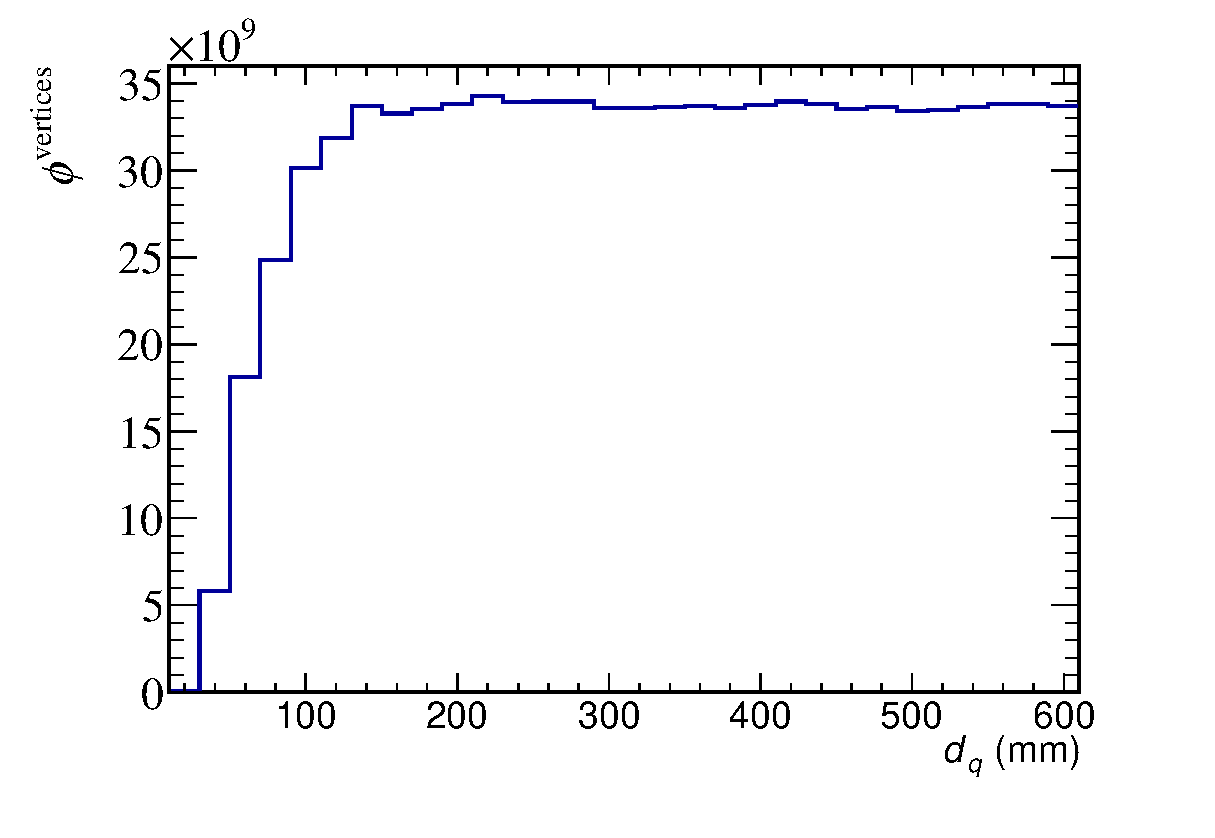
\includegraphics[width=9cm]{images/selection/vertex_recon/dq_marginalize} \label{fig:dqMarginalize}}
  \subfloat[$d_c$]{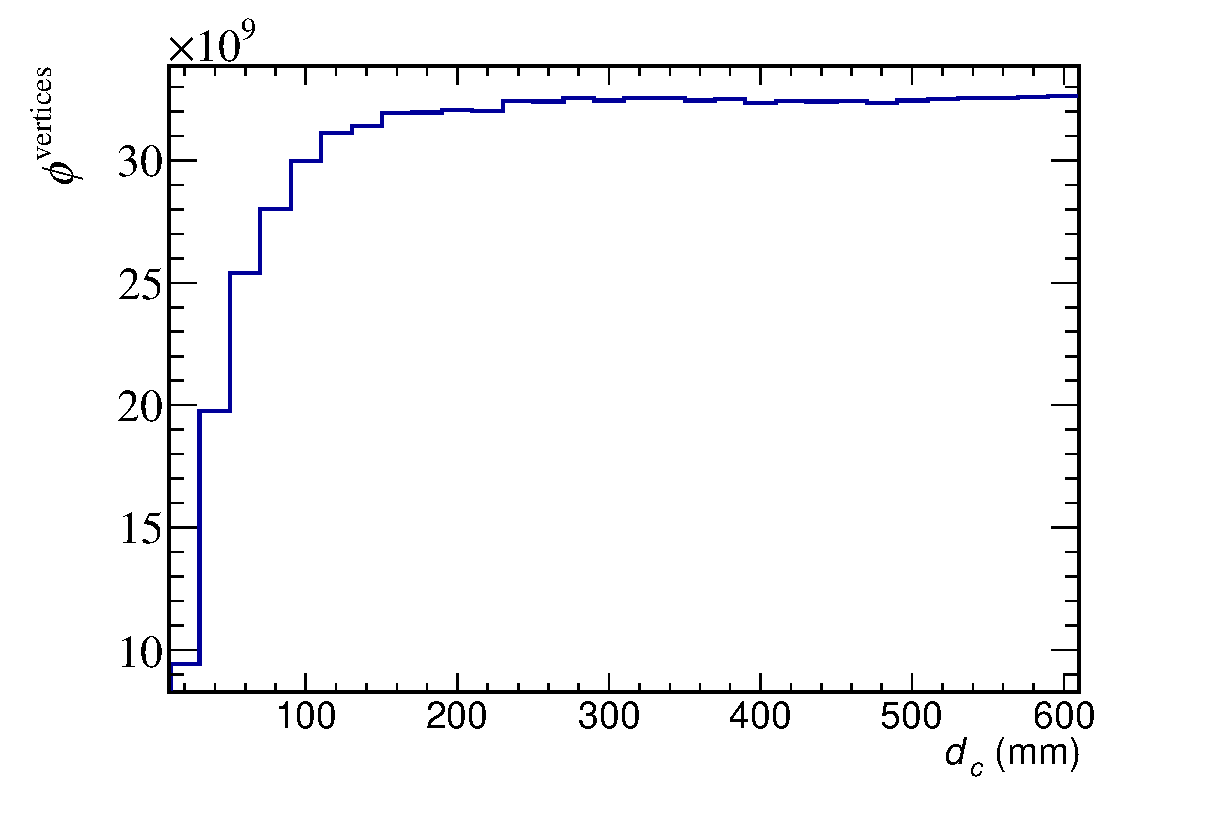
\includegraphics[width=9cm]{images/selection/vertex_recon/dc_marginalize} \label{fig:dcMarginalize}}
  \caption{$\phi^{\textrm{vertices}}$ vs the marginalized vertex reconstruction parameters.}
  \label{fig:VertexReconMarginalizedDistributions}
\end{figure}
By mapping out $\phi^{\textrm{vertices}}$ in ($d_q$,$d_c$) space, information about the preferred values of $d_q$ and $d_c$ can be found.  This space is shown in Fig.~\ref{fig:VertexReconFOM}.  It is clear from Fig.~\ref{fig:VertexReconFOM} that there is no clear maximum, but rather a plateau of  $\phi^{\textrm{vertices}}$ for $d_q$ and $d_c$ greater than 140 mm.  So, marginalized distributions of $d_q$ and $d_c$ can be produced to find where $\phi^{\textrm{vertices}}$ approaches zero which are shown in Fig.~\ref{fig:dqMarginalize} and Fig.~\ref{fig:dcMarginalize} respectively.  The values chosen are shown in table~\ref{table:VertexReconParameters}. 
\begin{table}[b!]
  \begin{tabular}{ c c }
    $\phi_d$ & $\phi_c$ \\ \hline \hline
    140 mm &  200 mm \\
  \end{tabular}
  \caption{Parameters for the vertex reconstruction in the ECal.}
  \label{table:VertexReconParameters}
\end{table}
The reconstruction now assesses the quality the crossings and then attempts to cluster the good quality crossings together to form vertex candidates.  The final step is to use the constituent tracks of each vertex candidate in a fit to estimate the position of the vertex.  The following method was proposed by X. Lu.  The position of the vertex, $\vec{P}$, is defined such that the sum of the squares of the distance of each track to $\vec{P}$ is minimised.  An example setup of this is shown in Fig.~\ref{fig:VertexVectorDiagram} for three constituent tracks.  By defining the square of the of the distance of a line, $l_i$, to $\vec{P}$ as $|\vec{r}_i|^2$, the function to minimise is
\begin{equation}
  D = \sum_i |\vec{r}_i|^2.
  \label{eqn:SumOfSquares}
\end{equation}
$\vec{P}$ is then defined as the point in space which satisfies
\begin{equation}
  \frac{\partial D}{\partial x} = \frac{\partial D}{\partial y} = \frac{\partial D}{\partial z} = 0.
  \label{eqn:SumOfSquaresMinCondition}
\end{equation}
The value of $|\vec{r}_i|$ is trivially defined by simple vector properties as 
\begin{equation}
  |\vec{r}_i| = \frac{|(\vec{P} - \vec{a}_i) \cross \vec{v}_i|}{|\vec{v}_i|} = |(\vec{P} - \vec{a}_i) \cross \hat{v}_i|,
  \label{eqn:DistanceOfPointToLine}
\end{equation}
where $\vec{v}_i$ is the direction vector of $\vec{l}_i$ and $\vec{a}_i$ is a point along $\vec{l}_i$.

\begin{figure}
  \centering
  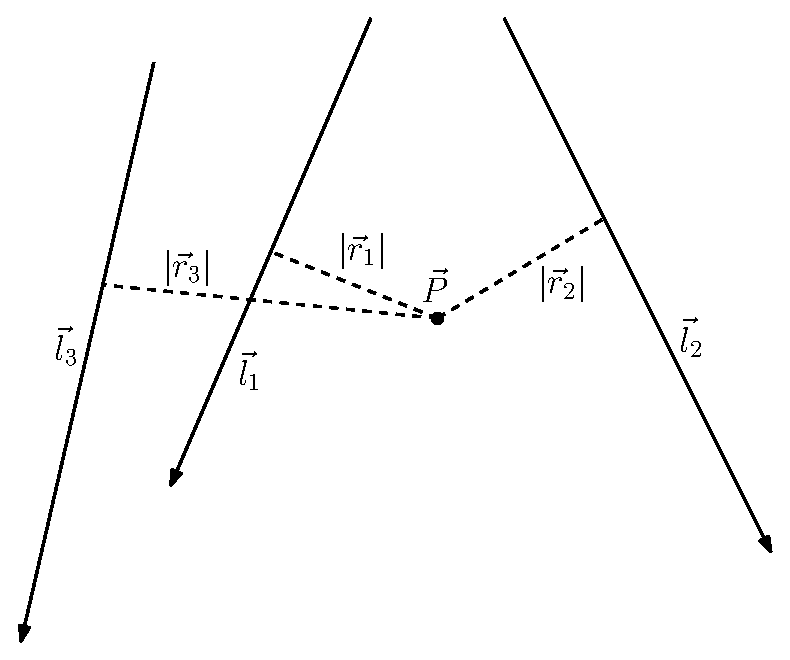
\includegraphics[width=8cm]{images/selection/vertex_recon/vertex_vector_diagram}
  \caption{Example of the vertex position, $\vec{P}$ for three lines: $\vec{l}_1$, $\vec{l}_2$ and $\vec{l}_3$. $|\vec{r}_1|$, $|\vec{r}_2|$ and $|\vec{r}_3|$ are the perpendicular distances of $\vec{l}_1$, $\vec{l}_2$ and $\vec{l}_3$ to $\vec{P}$ respectively.}
  \label{fig:VertexVectorDiagram}
\end{figure}


%\section{Data selection}
%Data flags

\section{Monte Carlo selection}
Make the cuts

\section{Properties of events in selection}

